% Options for packages loaded elsewhere
\PassOptionsToPackage{unicode}{hyperref}
\PassOptionsToPackage{hyphens}{url}
%
\documentclass[
]{book}
\usepackage{amsmath,amssymb}
\usepackage{lmodern}
\usepackage{ifxetex,ifluatex}
\ifnum 0\ifxetex 1\fi\ifluatex 1\fi=0 % if pdftex
  \usepackage[T1]{fontenc}
  \usepackage[utf8]{inputenc}
  \usepackage{textcomp} % provide euro and other symbols
\else % if luatex or xetex
  \usepackage{unicode-math}
  \defaultfontfeatures{Scale=MatchLowercase}
  \defaultfontfeatures[\rmfamily]{Ligatures=TeX,Scale=1}
\fi
% Use upquote if available, for straight quotes in verbatim environments
\IfFileExists{upquote.sty}{\usepackage{upquote}}{}
\IfFileExists{microtype.sty}{% use microtype if available
  \usepackage[]{microtype}
  \UseMicrotypeSet[protrusion]{basicmath} % disable protrusion for tt fonts
}{}
\makeatletter
\@ifundefined{KOMAClassName}{% if non-KOMA class
  \IfFileExists{parskip.sty}{%
    \usepackage{parskip}
  }{% else
    \setlength{\parindent}{0pt}
    \setlength{\parskip}{6pt plus 2pt minus 1pt}}
}{% if KOMA class
  \KOMAoptions{parskip=half}}
\makeatother
\usepackage{xcolor}
\IfFileExists{xurl.sty}{\usepackage{xurl}}{} % add URL line breaks if available
\IfFileExists{bookmark.sty}{\usepackage{bookmark}}{\usepackage{hyperref}}
\hypersetup{
  pdftitle={MATH3014-6027 Design (and Analysis) of Experiments},
  pdfauthor={Dave Woods},
  hidelinks,
  pdfcreator={LaTeX via pandoc}}
\urlstyle{same} % disable monospaced font for URLs
\usepackage{color}
\usepackage{fancyvrb}
\newcommand{\VerbBar}{|}
\newcommand{\VERB}{\Verb[commandchars=\\\{\}]}
\DefineVerbatimEnvironment{Highlighting}{Verbatim}{commandchars=\\\{\}}
% Add ',fontsize=\small' for more characters per line
\usepackage{framed}
\definecolor{shadecolor}{RGB}{248,248,248}
\newenvironment{Shaded}{\begin{snugshade}}{\end{snugshade}}
\newcommand{\AlertTok}[1]{\textcolor[rgb]{0.94,0.16,0.16}{#1}}
\newcommand{\AnnotationTok}[1]{\textcolor[rgb]{0.56,0.35,0.01}{\textbf{\textit{#1}}}}
\newcommand{\AttributeTok}[1]{\textcolor[rgb]{0.77,0.63,0.00}{#1}}
\newcommand{\BaseNTok}[1]{\textcolor[rgb]{0.00,0.00,0.81}{#1}}
\newcommand{\BuiltInTok}[1]{#1}
\newcommand{\CharTok}[1]{\textcolor[rgb]{0.31,0.60,0.02}{#1}}
\newcommand{\CommentTok}[1]{\textcolor[rgb]{0.56,0.35,0.01}{\textit{#1}}}
\newcommand{\CommentVarTok}[1]{\textcolor[rgb]{0.56,0.35,0.01}{\textbf{\textit{#1}}}}
\newcommand{\ConstantTok}[1]{\textcolor[rgb]{0.00,0.00,0.00}{#1}}
\newcommand{\ControlFlowTok}[1]{\textcolor[rgb]{0.13,0.29,0.53}{\textbf{#1}}}
\newcommand{\DataTypeTok}[1]{\textcolor[rgb]{0.13,0.29,0.53}{#1}}
\newcommand{\DecValTok}[1]{\textcolor[rgb]{0.00,0.00,0.81}{#1}}
\newcommand{\DocumentationTok}[1]{\textcolor[rgb]{0.56,0.35,0.01}{\textbf{\textit{#1}}}}
\newcommand{\ErrorTok}[1]{\textcolor[rgb]{0.64,0.00,0.00}{\textbf{#1}}}
\newcommand{\ExtensionTok}[1]{#1}
\newcommand{\FloatTok}[1]{\textcolor[rgb]{0.00,0.00,0.81}{#1}}
\newcommand{\FunctionTok}[1]{\textcolor[rgb]{0.00,0.00,0.00}{#1}}
\newcommand{\ImportTok}[1]{#1}
\newcommand{\InformationTok}[1]{\textcolor[rgb]{0.56,0.35,0.01}{\textbf{\textit{#1}}}}
\newcommand{\KeywordTok}[1]{\textcolor[rgb]{0.13,0.29,0.53}{\textbf{#1}}}
\newcommand{\NormalTok}[1]{#1}
\newcommand{\OperatorTok}[1]{\textcolor[rgb]{0.81,0.36,0.00}{\textbf{#1}}}
\newcommand{\OtherTok}[1]{\textcolor[rgb]{0.56,0.35,0.01}{#1}}
\newcommand{\PreprocessorTok}[1]{\textcolor[rgb]{0.56,0.35,0.01}{\textit{#1}}}
\newcommand{\RegionMarkerTok}[1]{#1}
\newcommand{\SpecialCharTok}[1]{\textcolor[rgb]{0.00,0.00,0.00}{#1}}
\newcommand{\SpecialStringTok}[1]{\textcolor[rgb]{0.31,0.60,0.02}{#1}}
\newcommand{\StringTok}[1]{\textcolor[rgb]{0.31,0.60,0.02}{#1}}
\newcommand{\VariableTok}[1]{\textcolor[rgb]{0.00,0.00,0.00}{#1}}
\newcommand{\VerbatimStringTok}[1]{\textcolor[rgb]{0.31,0.60,0.02}{#1}}
\newcommand{\WarningTok}[1]{\textcolor[rgb]{0.56,0.35,0.01}{\textbf{\textit{#1}}}}
\usepackage{longtable,booktabs,array}
\usepackage{calc} % for calculating minipage widths
% Correct order of tables after \paragraph or \subparagraph
\usepackage{etoolbox}
\makeatletter
\patchcmd\longtable{\par}{\if@noskipsec\mbox{}\fi\par}{}{}
\makeatother
% Allow footnotes in longtable head/foot
\IfFileExists{footnotehyper.sty}{\usepackage{footnotehyper}}{\usepackage{footnote}}
\makesavenoteenv{longtable}
\usepackage{graphicx}
\makeatletter
\def\maxwidth{\ifdim\Gin@nat@width>\linewidth\linewidth\else\Gin@nat@width\fi}
\def\maxheight{\ifdim\Gin@nat@height>\textheight\textheight\else\Gin@nat@height\fi}
\makeatother
% Scale images if necessary, so that they will not overflow the page
% margins by default, and it is still possible to overwrite the defaults
% using explicit options in \includegraphics[width, height, ...]{}
\setkeys{Gin}{width=\maxwidth,height=\maxheight,keepaspectratio}
% Set default figure placement to htbp
\makeatletter
\def\fps@figure{htbp}
\makeatother
\setlength{\emergencystretch}{3em} % prevent overfull lines
\providecommand{\tightlist}{%
  \setlength{\itemsep}{0pt}\setlength{\parskip}{0pt}}
\setcounter{secnumdepth}{5}
\usepackage{booktabs}
\ifluatex
  \usepackage{selnolig}  % disable illegal ligatures
\fi
\usepackage[]{natbib}
\bibliographystyle{apalike}

\title{MATH3014-6027 Design (and Analysis) of Experiments}
\author{Dave Woods}
\date{2022-02-01}

\usepackage{amsthm}
\newtheorem{theorem}{Theorem}[chapter]
\newtheorem{lemma}{Lemma}[chapter]
\newtheorem{corollary}{Corollary}[chapter]
\newtheorem{proposition}{Proposition}[chapter]
\newtheorem{conjecture}{Conjecture}[chapter]
\theoremstyle{definition}
\newtheorem{definition}{Definition}[chapter]
\theoremstyle{definition}
\newtheorem{example}{Example}[chapter]
\theoremstyle{definition}
\newtheorem{exercise}{Exercise}[chapter]
\theoremstyle{definition}
\newtheorem{hypothesis}{Hypothesis}[chapter]
\theoremstyle{remark}
\newtheorem*{remark}{Remark}
\newtheorem*{solution}{Solution}
\begin{document}
\maketitle

{
\setcounter{tocdepth}{1}
\tableofcontents
}
\hypertarget{preface}{%
\chapter*{Preface}\label{preface}}
\addcontentsline{toc}{chapter}{Preface}

These are draft lecture notes for the modules MATH3014 and MATH6027 Design (and Analysis) of Experiments at the University of Southampton for academic year 2021-22. They are very much work in progress.

\newcommand{\bx}{\boldsymbol{x}}
\newcommand{\btheta}{\boldsymbol{\theta}}
\newcommand{\bbeta}{\boldsymbol{\beta}}
\newcommand{\bvarepsilon}{\boldsymbol{\varepsilon}}
\newcommand{\by}{\boldsymbol{y}}
\newcommand{\rT}{\mathrm{T}}
\newcommand{\Var}{\operatorname{Var}}
\newcommand{\bY}{\boldsymbol{y}}
\newcommand{\btau}{\boldsymbol{\tau}}

\hypertarget{intro}{%
\chapter{Motivation, introduction and revision}\label{intro}}

\begin{definition}
\protect\hypertarget{def:exp}{}\label{def:exp}

An \textbf{experiment} is the process through which data are collected to answer a scientific question (physical science, social science, actuarial science \(\dots\)) by \textbf{deliberately} varying some features of the process under study in order to understand the impact of these changes on measureable responses.

In this course we consider only \emph{intervention} experiments, in which some aspects of the process are under the experimenters' control. We do not consider \emph{surveys} or \emph{observational} studies.

\end{definition}

\begin{definition}
\protect\hypertarget{def:design}{}\label{def:design}

\textbf{Design of experiments} is the topic in Statistics concerned with the selection of settings of controllable variables or factors in an experiment and their allocation to experimental units in order to maximise the effectiveness of the experiment at achieving its aim.

\end{definition}

People have been designing experiments for as long as they have been exploring the natural world. Some notable milestones in the history of the design of experiments include:

\begin{itemize}
\tightlist
\item
  prior to the 20th century:

  \begin{itemize}
  \tightlist
  \item
    \href{https://en.wikipedia.org/wiki/Baconian_method}{Francis Bacon} (17th century; pioneer of the experimental methods)
  \item
    \href{https://en.wikipedia.org/wiki/James_Lind}{James Lind} (18th century; experiments to eliminate scurvy)
  \item
    \href{https://en.wikipedia.org/wiki/Charles_Sanders_Peirce\#Probability_and_statistics}{Charles Peirce} (19th century; advocated randomised experiments and randomisation-based inference)
  \end{itemize}
\item
  1920s: agriculture (particularly at the \href{https://www.rothamsted.ac.uk/history-and-heritage}{Rothamsted Agricultural Research Station})
\item
  1940s: clinical trials (\href{https://en.wikipedia.org/wiki/Austin_Bradford_Hill}{Austin Bradford-Hill})
\item
  1950s: (manufacturing) industry (\href{https://en.wikipedia.org/wiki/W._Edwards_Deming}{W. Edwards Deming}; \href{https://en.wikipedia.org/wiki/Genichi_Taguchi}{Genichi Taguchi})
\item
  1960s: psychology and economics (\href{https://en.wikipedia.org/wiki/Vernon_L._Smith}{Vernon Smith})
\item
  1980s: in-silico (\href{https://en.wikipedia.org/wiki/Computer_experiment}{computer experiments})
\item
  2000s: online (\href{https://en.wikipedia.org/wiki/A/B_testing}{A/B testing})
\end{itemize}

See \citet{LB2020} for further history, anecdotes and examples, especially from psychology and technology.

Figure \ref{fig:broadbalk} shows the \href{http://www.era.rothamsted.ac.uk/Broadbalk}{Broadbalk} agricultural field experiment at Rothamsted, one of the longest continuous running experiments in the world, which is testing the impact of different manures and fertilizers on the growth of winter wheat.

\begin{figure}
 
 {\centering 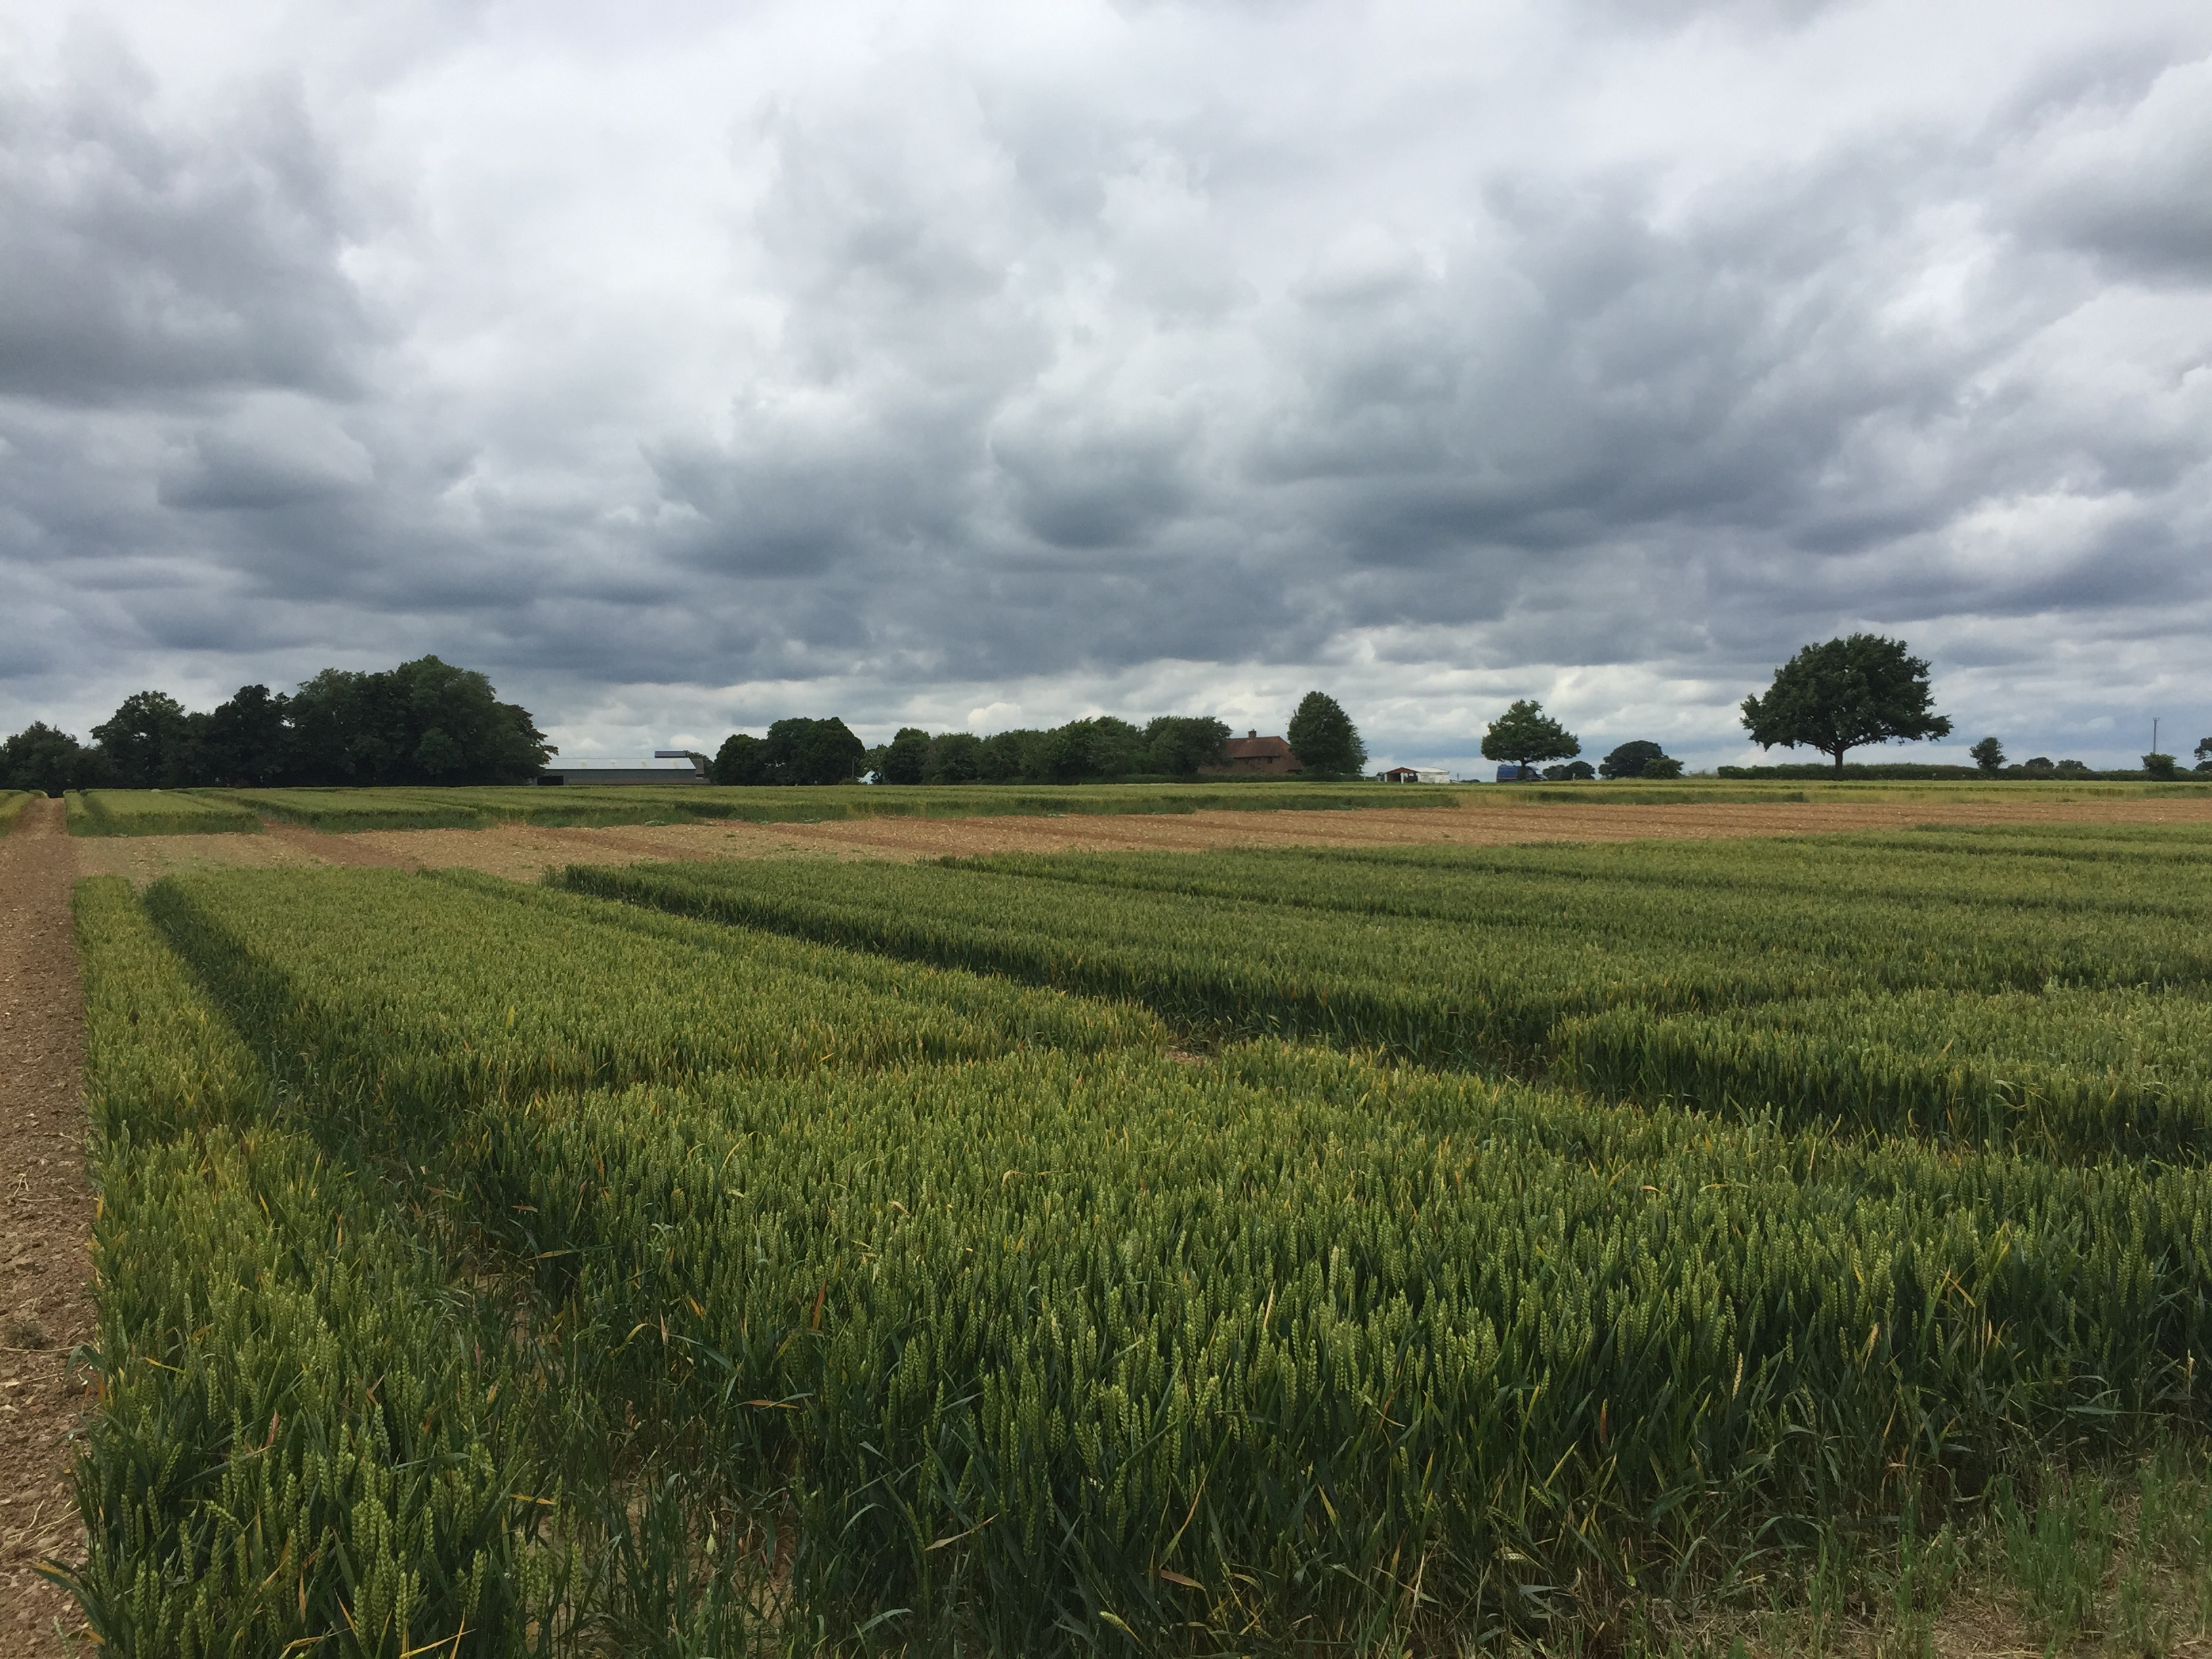
\includegraphics[width=0.75\linewidth]{figures/broadbalk} 
 
 }
 
 \caption{The Broadbalk experiment, Rothamsted (photograph taken 2016)}\label{fig:broadbalk}
 \end{figure}

\hypertarget{motivation}{%
\section{Motivation}\label{motivation}}

\begin{example}
\protect\hypertarget{exm:motivation}{}\label{exm:motivation}

Consider an experiment to compare two treatments (e.g.~drugs, diets, fertilisers, \(\dots\)). We have \(n\) subjects (people, mice, plots of land, \(\dots\)), each of which can be assigned one of the two treatments. A response (protein measurement, weight, yield, \(\dots\)) is then measured.

\end{example}

\textbf{Question:} How many subjects should be assigned to each treatment to gain the most precise\footnote{Smallest variance.} inference about the difference in response from the two treatments?

Consider a linear statistical model\footnote{In this course, we will almost always start with a statistical model which we wish to use to answer our scientific question.} for the response (see MATH2010):

\begin{equation}
Y_j=\beta_{0}+\beta_{1}x_j+\varepsilon_j\,,\qquad j=1, \ldots, n\,,
\label{eq:slr}
\end{equation}

where \(\varepsilon_j\sim N(0,\sigma^{2})\) are independent and identically distributed errors and \(\beta_{0}, \beta_{1}\) are unknown constants (parameters).

Let\footnote{Other codings can be used: e.g. 0,1; see later in the module. It makes no difference for our current purpose.}
\begin{equation}
x_{j}=\left\{\begin{array}{ll}
-1&\textrm{if treatment 1 is applied to the $j$th subject}\\
+1&\textrm{if treatment 2 is applied to the $j$th subject}\nonumber ,
\end{array}
\right.
\end{equation}
for \(j=1,\dots,n\).\footnote{We will discuss the choice of \emph{coding} -1, +1 later.}

The difference in expected response from treatments 1 and 2 is

\begin{equation}
\begin{split}
\textrm{E}[Y_j\, |\, x_j = +1] - \textrm{E}[Y_j\, |\, x_j = -1] & = \beta_{0}+\beta_{1}-\beta_{0}+\beta_{1} \\
& = 2\beta_{1}\,.
\end{split}
\label{eq:ex-ex-response}
\end{equation}

Therefore, we require the the most precise estimator of \(\beta_{1}\) possible. That is, we wish to make the variance of our estimator of \(\beta_1\) as small as possible.

Parameters \(\beta_{0}\) and \(\beta_{1}\) can be estimated using least squares (see MATH2010). For \(Y_1,\dots,Y_n\), we can write the model down in matrix form:

\begin{equation*}
\left[ \begin{array}{c}
Y_1\\
\vdots\\
Y_n\end{array}\right]
=\left[ \begin{array}{cc}
1&x_{1}\\
\vdots&\vdots\\
1&x_{n}\end{array}\right]
\left[ \begin{array}{c}
\beta_{0}\\
\beta_{1}\end{array}\right]
+\left[ \begin{array}{c}
\varepsilon_{1}\\
\vdots\\
\varepsilon_{n}\end{array}\right]\,.
\end{equation*}

Or, by defining some notation:

\begin{equation}
\boldsymbol{Y}=X\boldsymbol{\beta}+\boldsymbol{\varepsilon}\,
\label{eq:matrix-model}
\end{equation}

where

\begin{itemize}
\tightlist
\item
  \(\boldsymbol{Y}\) - \(n\times 1\) vector of responses;
\item
  \(X\) - \(n\times p\) model matrix;
\item
  \(\boldsymbol{\beta}\) - \(p\times 1\) vector of parameters;
\item
  \(\boldsymbol{\varepsilon}\) - \(n\times 1\) vector of errors.
\end{itemize}

The \textbf{least squares estimators}, \(\hat{\boldsymbol{\beta}}\), are chosen such that the quadratic form

\begin{equation*}
(\boldsymbol{Y}-X\boldsymbol{\beta})^{\textrm{T}}(\boldsymbol{Y}-X\boldsymbol{\beta})
\end{equation*}

is minimised (recall that \(\textrm{E}(\textbf{Y})=X\boldsymbol{\beta}\)). Therefore

\begin{equation*}
\hat{\boldsymbol{\beta}} = \textrm{argmin}_{\boldsymbol{\beta}}(\boldsymbol{Y}^{\textrm{T}}\boldsymbol{Y}+\boldsymbol{\beta}^{\textrm{T}}X^{\textrm{T}}X\boldsymbol{\beta}
-2\boldsymbol{\beta}^{\textrm{T}}X^{\textrm{T}}\boldsymbol{Y})\,.
\end{equation*}

If we differentiate with respect to \(\boldsymbol{\beta}\)\footnote{Check the \href{https://www.math.uwaterloo.ca/~hwolkowi/matrixcookbook.pdf}{Matrix Cookbook} for matrix calculus, amongst much else.},

\begin{equation*}
\frac{\partial}{\partial\boldsymbol{\beta}}=2X^{\textrm{T}}X\boldsymbol{\beta}-2X^{\textrm{T}}\boldsymbol{Y}\,,\nonumber
\end{equation*}

and equate to 0, we get the estimators

\begin{equation}
\hat{\boldsymbol{\beta}}=(X^{\textrm{T}}X)^{-1}X^{\textrm{T}}\boldsymbol{Y}\,.
\label{eq:lsestimators}
\end{equation}

These are the least squares estimators.

For Example \ref{exm:motivation},

\[
X=\left[\begin{array}{cc}
1&x_{1}\\
\vdots&\vdots\\
1&x_{n}\end{array}\right]\,,
\qquad
X^{\textrm{T}}X=\left[\begin{array}{cc}
n&\sum x_j\\
\sum x_j&\sum x_j^{2}\end{array}\right]\,,
\]

\[
(X^{\textrm{T}}X)^{-1}=\frac{1}{n\sum x_j^{2}-(\sum x_j)^{2}}\left[\begin{array}{cc}
\sum x_j^{2}&-\sum x_j\\
-\sum x_j&n\end{array}\right]\,,
\qquad
X^{\textrm{T}}\boldsymbol{Y}=\left[\begin{array}{c}
\sum Y_j\\
\sum x_jY_j\end{array}\right]\,.
\]
Then,
\begin{align}
\hat{\boldsymbol{\beta}}=\left[\begin{array}{c}
\hat{\beta}_{0}\\
\hat{\beta}_{1}\end{array}\right]
& =\frac{1}{n\sum x_j^{2}-(\sum x_j)^{2}}
\left[\begin{array}{cc}
\sum x_j^{2}&-\sum x_j\\
-\sum x_j&n\end{array}\right]
\left[\begin{array}{c}
\sum Y_j\\
\sum x_jY_j\end{array}\right]\nonumber \\
&= \frac{1}{n\sum x_j^{2}-(\sum x_j)^{2}}\left[\begin{array}{c}
\sum Y_j\sum x_j^{2}-\sum x_j\sum x_jY_j\\
n\sum x_jY_j-\sum x_j\sum Y_j\end{array}\right]\,.
\end{align}

We don't usually work through the algebra in such detail; the matrix form is often sufficient for theoretical and numerical calculations and software, e.g.~\texttt{R}, can be used.

The precision of \(\hat{\boldsymbol{\beta}}\) is measured via the variance-covariance matrix, given by
\begin{align}
\textrm{Var}(\hat{\boldsymbol{\beta}}) & = \textrm{Var}\{(X^{\textrm{T}}X)^{-1}X^{\textrm{T}}\boldsymbol{Y}\}\\
& =(X^{\textrm{T}}X)^{-1}X^{\textrm{T}}\textrm{Var}(\boldsymbol{Y})X(X^{\textrm{T}}X)^{-1}\\
& = (X^{\textrm{T}}X)^{-1}\sigma^{2}\,,
\end{align}

where \(\boldsymbol{Y}\sim N(X\boldsymbol{\beta},I_n\sigma^{2})\), where \(I_n\) is an \(n\times n\) identity matrix.

Hence, in our example,
\begin{align*}
\textrm{Var}(\hat{\boldsymbol{\beta}}) & = \frac{1}{n\sum x_j^{2}-(\sum x_j)^{2}}\left[\begin{array}{cc}
\sum x_j^{2}&-\sum x_j\\
-\sum x_j&n\end{array}\right]\sigma^{2}\\
& = \left[\begin{array}{cc}
\textrm{Var}(\hat\beta_{0})&\textrm{Cov}(\hat\beta_{0},\hat\beta_{1})\\
\textrm{Cov}(\hat\beta_{0},\hat\beta_{1})&\textrm{Var}(\hat\beta_{1})\end{array}\right]\,.
\end{align*}

For estimating the difference between treatments, we are interested in

\begin{align*}
\textrm{Var}(\hat{\beta}_{1})& = \frac{n}{n\sum x_j^{2}-(\sum x_j)^{2}}\sigma^{2}\\
 & = \frac{n}{n^2 - (\sum x_j)^2}\sigma^{2}\,,
\end{align*}
as \(x_j=\pm 1\), therefore \(x_j^2=1\) for all \(j=1,\ldots,n\), and hence \(\sum x_j^2=n\).

To achieve the most precise estimator, we need to minimise \(\textrm{Var}(\hat{\beta}_{1})\) or equivalently minimise \(|\sum x_j|\). This goal can achieve this through the choice of \(x_{1},\dots,x_{n}\):

\begin{itemize}
\tightlist
\item
  as each \(x_j\) can only take one of two values, -1 or +1, this is equivalent to choosing the numbers of subjects assigned to treatment 1 and treatment 2;
\item
  call these \(n_{1}\) and \(n_{2}\) respectively, with \(n_{1}+n_{2}=n\)
\end{itemize}

It is obvious that \(\sum x_j = 0\) if and only if \(n_1=n_2\). Therefore, assuming \(n\) is even, the \textbf{optimal design} has

\begin{itemize}
\tightlist
\item
  \(n_{1}=\frac{n}{2}\) subjects assigned to treatment 1 and
\item
  \(n_{2}=\frac{n}{2}\) subjects assigned to treatment 2.
\end{itemize}

For \(n\) odd, we choose \(n_{1}=\frac{n+1}{2}\), \(n_{2}=\frac{n-1}{2}\), or vice versa.

\begin{definition}
\protect\hypertarget{def:simple-efficiency}{}\label{def:simple-efficiency}

We can assess different designs using their \textbf{efficiency}:
\begin{equation}
\textrm{Eff}=\frac{\textrm{Var}(\hat{\beta}_{1}\, |\, d^{*})}{\textrm{Var}(\hat{\beta}_{1}\, |\, d_{1})}
\label{eq:simple-efficiency}
\end{equation}

where \(d_{1}\) is a design we want to assess and \(d^{*}\) is the optimal design with smallest variance. Note that \(0\leq\textrm{Eff}\leq 1\).

\end{definition}

In Figure \ref{fig:simple-efficiency} below, we plot this efficiency for Example \ref{exm:motivation}, using different choices of \(n_1\). The total number of runs is fixed at \(n = 100\), and the function \texttt{eff} calculates the efficiency from Definition \ref{def:simple-efficiency} for a design with \(n_1\) subjects assigned to treatment 1. Clearly, efficiency of 1 is achieved when \(n_1 = n_2\) (equal allocation of treatments 1 and 2). If \(n_1=0\) or \(n_1 = 1\), the efficiency is zero; we cannot estimate the difference between two treatments if we only allocate subjects to one of them.



\begin{Shaded}
\begin{Highlighting}[]
\NormalTok{n }\OtherTok{\textless{}{-}} \DecValTok{100} 
\NormalTok{eff }\OtherTok{\textless{}{-}} \ControlFlowTok{function}\NormalTok{(n1) }\DecValTok{1} \SpecialCharTok{{-}}\NormalTok{ ((}\DecValTok{2} \SpecialCharTok{*}\NormalTok{ n1 }\SpecialCharTok{{-}}\NormalTok{ n) }\SpecialCharTok{/}\NormalTok{ n)}\SpecialCharTok{\^{}}\DecValTok{2} 
\FunctionTok{curve}\NormalTok{(eff, }\AttributeTok{from =} \DecValTok{0}\NormalTok{, }\AttributeTok{to =}\NormalTok{ n, }\AttributeTok{ylab =} \StringTok{"Eff"}\NormalTok{, }\AttributeTok{xlab =} \FunctionTok{expression}\NormalTok{(n[}\DecValTok{1}\NormalTok{]))}
\end{Highlighting}
\end{Shaded}

\begin{figure}
\centering
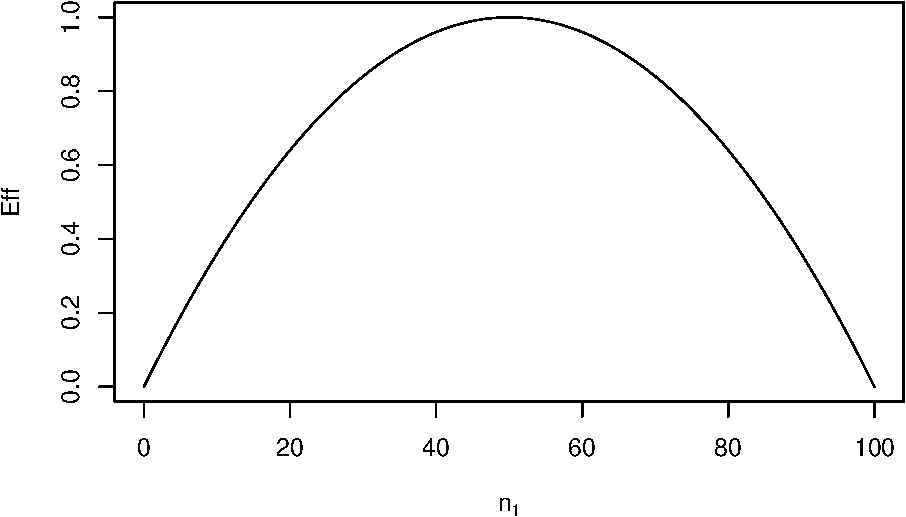
\includegraphics{bookdown_math3014-6027_files/figure-latex/simple-efficiency-1.pdf}
\caption{\label{fig:simple-efficiency}Efficiencies for designs for Example \ref{exm:motivation} with different numbers, \(n_1\), of subjects assigned to treatment 1 when the total number of subjects is \(n=100\).}
\end{figure}

\hypertarget{aims-of-experimentation-and-some-examples}{%
\section{Aims of experimentation and some examples}\label{aims-of-experimentation-and-some-examples}}

Some reasons experiments are performed:

\begin{enumerate}
\def\labelenumi{\arabic{enumi}.}
\tightlist
\item
  Treatment comparison (Chapters 2 and 3)
\end{enumerate}

\begin{itemize}
\tightlist
\item
  compare several treatments (and choose the best)
\item
  e.g.~clinical trial, agricultural field trial
\end{itemize}

\begin{enumerate}
\def\labelenumi{\arabic{enumi}.}
\setcounter{enumi}{1}
\tightlist
\item
  Factor screening (Chapters 4, 5 and 6)
\end{enumerate}

\begin{itemize}
\tightlist
\item
  many complex systems may involve a large number of (discrete) factors (controllable features)
\item
  which of these factors have a substantive impact?
\item
  (relatively) small experiments
\item
  e.g.~industrial experiments on manufacturing processes
\end{itemize}

\begin{enumerate}
\def\labelenumi{\arabic{enumi}.}
\setcounter{enumi}{2}
\tightlist
\item
  Response surface exploration (Chapter 7)
\end{enumerate}

\begin{itemize}
\tightlist
\item
  detailed description of relationship between important (continuous) variables and response
\item
  typically second order polynomial regression models
\item
  larger experiments, often built up sequentially
\item
  e.g.~alcohol yields in a pharmaceutical experiments
\end{itemize}

\begin{enumerate}
\def\labelenumi{\arabic{enumi}.}
\setcounter{enumi}{3}
\tightlist
\item
  Optimisation (Chapter 7)
\end{enumerate}

\begin{itemize}
\tightlist
\item
  finding settings of variables that lead to maximum or minimum response
\item
  typically use response surface methods and sequential ``hill climbing'\,' strategy
\end{itemize}

\hypertarget{some-definitions}{%
\section{Some definitions}\label{some-definitions}}

\begin{definition}
\protect\hypertarget{def:response}{}\label{def:response}

The \textbf{response} \(Y\) is the outcome measured in an experiment; e.g.~yield from a chemical process. The response from the \(n\) observations are denoted \(Y_{1},\dots,Y_{n}\).

\end{definition}

\begin{definition}
\protect\hypertarget{def:factor-variable}{}\label{def:factor-variable}

\textbf{Factors} (discrete) or \textbf{variables} (continuous) are features which can be set or controlled in an experiment; \(m\) denotes the number of factors or variables under investigation. For discrete factors, we call the possible settings of the factor its \textbf{levels}. We denote by \(x_{ij}\) the value taken by factor or variable \(i\) in the \(j\)th run of the experiment (\(i = 1, \ldots, m\); \(j = 1, \ldots, n\)).

\end{definition}

\begin{definition}
\protect\hypertarget{def:treatment}{}\label{def:treatment}

The \textbf{treatments} or \textbf{support points} are the \emph{distinct} combinations of factor or variable values in the experiment.

\end{definition}

\begin{definition}
\protect\hypertarget{def:unit}{}\label{def:unit}

An experimental \textbf{unit} is the basic element (material, animal, person, time unit, \ldots) to which a treatment can be applied to produce a response.

\end{definition}

In Example \ref{exm:motivation} (comparing two treatments):

\begin{itemize}
\tightlist
\item
  Response \(Y\): Measured outcome, e.g.~protein level or pain score in clinical trial, yield in an agricultural field trial.
\item
  Factor \(x\): ``treatment'' applied
\item
  Levels
  \[
  \begin{array}{ll}
  \textrm{treatment 1}&x =-1\\
  \textrm{treatment 2}&x =+1
  \end{array}
  \]
\item
  Treatment or support point: Two treatments or support points
\item
  Experimental unit: Subject (person, animal, plot of land, \ldots).
\end{itemize}

\hypertarget{principles}{%
\section{Principles of experimentation}\label{principles}}

Three fundamental principles that need to be considered when designing an experiment are:

\begin{itemize}
\tightlist
\item
  replication
\item
  randomisation
\item
  stratification (blocking)
\end{itemize}

\hypertarget{replication}{%
\subsection{Replication}\label{replication}}

Each treatment is applied to a number of experimental units, with the \(j\)th treatment replicated \(r_{j}\) times. This enables the estimation of the variances of treatment effect estimators; increasing the number of replications, or replicates, decreases the variance of estimators of treatment effects.
(Note: proper replication involves independent application of the treatment to different experimental units, not just taking several measurements from the same unit).

\hypertarget{randomisation}{%
\subsection{Randomisation}\label{randomisation}}

Randomisation should be applied to the allocation of treatments to units. Randomisation protects against \textbf{bias}; the effect of
variables that are unknown and potentially uncontrolled or
subjectivity in applying treatments. It also provides a formal basis
for inference and statistical testing.

For example, in a clinical trial to compare a new drug and a control random allocation protects against

\begin{itemize}
\tightlist
\item
  ``unmeasured and uncontrollable'' features (e.g.~age, sex, health)
\item
  bias resulting from the clinician giving new drug to patients who are sicker.
\end{itemize}

Clinical trials are usually also \emph{double-blinded}, i.e.~neither the healthcare professional nor the patient knows which treatment the patient is receiving.

\hypertarget{blocking}{%
\subsection{Stratification (or blocking)}\label{blocking}}

We would like to use a wide variety of experimental units (e.g.~people or plots of land) to ensure \textbf{coverage} of our results, i.e.~validity of our conclusions across the population of interest. However, if the sample of units from the population is too heterogenous, then this will induce too much random variability, i.e.~increase \(\sigma^{2}\) in \(\varepsilon_{j}\sim N(0,\sigma^{2})\), and hence increase the variance of our parameter estimators.

We can reduce this extraneous variation by splitting our units into homogenous sets, or \textbf{blocks}, and including a blocking term in the model. The simplest blocked experiment is a \textbf{randomised complete block design}, where each block contains enough units for all treatments to be applied. Comparisons can then be made \emph{within} each block.

Basic principle: block what you can, randomise what you cannot.

Later we will look at blocking in more detail, and the principle of \textbf{incomplete blocks}.

\hypertarget{lin-model-rev}{%
\section{Revision on the linear model}\label{lin-model-rev}}

Recall: \(\boldsymbol{Y}=X\boldsymbol{\beta}+\boldsymbol{\varepsilon}\), with \(\boldsymbol{\varepsilon}\sim N(\boldsymbol{0},I_n\sigma^{2})\). Let the \(j\)th row of \(X\) be denoted \(\boldsymbol{x}^\textrm{T}_j\), which holds the values of the predictors, or explanatory variables, for the \(j\)th observation. Then

\begin{equation*}
Y_j=\boldsymbol{x}_j^{\textrm{T}}\boldsymbol{\beta}+\varepsilon_j\,,\quad j=1,\ldots,n\,.
\end{equation*}

For example, quite commonly, for continuous variables

\[
\boldsymbol{x}_j=(1,x_{1j},x_{2j},\dots,x_{mj})^{\textrm{T}}\,,
\]

and so
\[
\boldsymbol{x}_j^{\textrm{T}}\boldsymbol{\beta}=\beta_{0}+\beta_{1}x_{1j}+\dots+\beta_{m}x_{mj}\,.
\]

The laest squares estimators are given by

\begin{equation}
\hat{\boldsymbol{\beta}}=(X^{\textrm{T}}X)^{-1}X^{\textrm{T}}\boldsymbol{Y}\,,\nonumber
\end{equation}

with

\begin{equation}
\textrm{Var}(\hat{\boldsymbol{\beta}})=(X^{\textrm{T}}X)^{-1}\sigma^{2}\,.\nonumber
\end{equation}

\hypertarget{variance-of-a-predictionfitted-value}{%
\subsection{Variance of a Prediction/Fitted Value}\label{variance-of-a-predictionfitted-value}}

A prediction of the mean response at point \(\boldsymbol{x}_0\) (which may or may not be in the design) is

\[
\hat{Y}_0 = \boldsymbol{x}_0^{\textrm{T}}\hat{\boldsymbol{\beta}}\,,
\]

with

\begin{align*}
\textrm{Var}(\hat{Y}_0) & = \textrm{Var}\left(\boldsymbol{x}_0^{\textrm{T}}\hat{\boldsymbol{\beta}}\right) \\
& = \boldsymbol{x}_0^{\textrm{T}}\textrm{Var}(\hat{\boldsymbol{\beta}})\boldsymbol{x}_0 \\
& = \boldsymbol{x}_0^{\textrm{T}}(X^{\textrm{T}}X)^{-1}\boldsymbol{x}_0\sigma^{2}\,.
\end{align*}

For a linear model, this variance depends only on the assumed regression model and the design (through \(X\)), the point at which prediction is to be made (\(\boldsymbol{x}_0\)) and the value of \(\sigma^2\); it does not depend on data \(\boldsymbol{Y}\) or parameters \(\boldsymbol{\beta}\).

Similarly, we can find the variance-covariance matrix of the fitted values:
\[
\textrm{Var}(\hat{Y})=\textrm{Var}(X\hat{\boldsymbol{\beta}})=X(X^{\textrm{T}}X)^{-1}X^{\textrm{T}}\sigma^{2}\,.
\]

\hypertarget{analysis-of-variance-and-r2-as-model-comparison}{%
\subsection{\texorpdfstring{Analysis of Variance and R\(^{2}\) as Model Comparison}{Analysis of Variance and R\^{}\{2\} as Model Comparison}}\label{analysis-of-variance-and-r2-as-model-comparison}}

To assess the goodness-of-fit of a model, we can use the residual sum of squares

\begin{align*}
\textrm{RSS} & = (\boldsymbol{Y} - X\hat{\boldsymbol{\beta}})^{\textrm{T}} (\boldsymbol{Y} - X\hat{\boldsymbol{\beta}})\\
& = \sum^{n}_{j=1}\left\{Y_{j}-\boldsymbol{x}_{j}^{\textrm{T}}\hat{\boldsymbol{\beta}}\right\}^{2}\\
& = \sum^{n}_{j=1}r_{j}^{2}\,,
\end{align*}

where

\[
r_{j}=Y_{j}-\boldsymbol{x}_{j}^{\textrm{T}}\hat{\boldsymbol{\beta}}\,.
\]

Often, a comparison is made to the null model

\[
Y_{j}=\beta_{0}+\varepsilon_{j}\,,
\]

i.e.~\(Y_{i}\sim N(\beta_{0},\sigma^{2})\). The residual sum of squares for the null model is given by

\[
\textrm{RSS}(\textrm{null}) = \boldsymbol{Y}^{\textrm{T}}\boldsymbol{Y} - m\bar{Y}^{2}\,,
\]
as

\[
\hat{\beta}_{0} = \bar{Y} = \frac{1}{n}\sum_{j=1}^n Y_{j}\,.
\]

How do we compare these models?

\begin{enumerate}
\def\labelenumi{\arabic{enumi}.}
\tightlist
\item
  Ratio of residual sum of squares:
  \begin{align*}
  R^{2} & = 1 - \frac{\textrm{RSS}}{\textrm{RSS}(\textrm{null})} \\
  & = 1 - \frac{(\boldsymbol{Y}-X\hat{\boldsymbol{\beta}})^{\textrm{T}}(\boldsymbol{Y}-X\hat{\boldsymbol{\beta}})}{\boldsymbol{Y}^{\textrm{T}}\boldsymbol{Y}-n\bar{Y}^{2}}\,.
  \end{align*}
\end{enumerate}

The quantity \(0\leq R^{2}\leq 1\) is sometimes called the \textbf{coefficient of multiple determination}:

\begin{itemize}
\tightlist
\item
  high \(R^{2}\) implies that the model describes much of the variation in the data;
\item
  \textbf{but} note that \(R^{2}\) will always increase as \(p\) (the number of explanatory variables) increases, with \(R^{2}=1\) when \(p=n\);
\item
  some software packages will report the adjusted \(R^{2}\).
\end{itemize}

\begin{align*}
R^{2}_{a} & = 1-\frac{\textrm{RSS}/(n-p)}{\textrm{RSS}(\textrm{null})/(n-1)}\\
& = 1 - \frac{(\boldsymbol{Y} - X\hat{\boldsymbol{\beta}})^{\textrm{T}} (\boldsymbol{Y} - X\hat{\boldsymbol{\beta}})/(n-p)}{(\boldsymbol{Y}^{\textrm{T}}\boldsymbol{Y} - n\bar{Y}^{2})/(n-1)};
\end{align*}

\begin{itemize}
\tightlist
\item
  \(R_a^2\) does not necessarily increase with \(p\) (as we divide by degrees of freedom to adjust for complexity of the model).
\end{itemize}

\begin{enumerate}
\def\labelenumi{\arabic{enumi}.}
\setcounter{enumi}{1}
\tightlist
\item
  Analysis of variance (ANOVA): An ANOVA table is compact way of presenting the results of (sequential) comparisons of nested models. You should be familiar with an ANOVA table of the following form.
\end{enumerate}

\begin{longtable}[]{@{}
  >{\raggedright\arraybackslash}p{(\columnwidth - 6\tabcolsep) * \real{0.25}}
  >{\raggedright\arraybackslash}p{(\columnwidth - 6\tabcolsep) * \real{0.25}}
  >{\raggedright\arraybackslash}p{(\columnwidth - 6\tabcolsep) * \real{0.25}}
  >{\raggedright\arraybackslash}p{(\columnwidth - 6\tabcolsep) * \real{0.25}}@{}}
\caption{\label{tab:anova} A standard ANOVA table.}\tabularnewline
\toprule
Source & Degress of Freedom & (Sequential) Sum of Squares & Mean Square \\
\midrule
\endfirsthead
\toprule
Source & Degress of Freedom & (Sequential) Sum of Squares & Mean Square \\
\midrule
\endhead
Regression & \(p-1\) & By subtraction; see \eqref{eq:SSS} & Reg SS/\((p-1)\) \\
Residual & \(n-p\) & \((\boldsymbol{Y}-X\hat{\boldsymbol{\beta}})^{\textrm{T}}(\boldsymbol{Y}-X\hat{\boldsymbol{\beta}})\)\footnote{Residual sum of squares for the full regression model.} & RSS/\((n-p)\) \\
Total & \(n-1\) & \(\boldsymbol{Y}^{\textrm{T}}\boldsymbol{Y}-n\bar{Y}^{2}\)\footnote{Residual sum of squares for the null model.} & \\
\bottomrule
\end{longtable}

In row 1 of Table \ref{tab:anova} above,
\begin{align}
\textrm{Regression SS = Total SS $-$ RSS} & = \boldsymbol{Y}^{\textrm{T}}\boldsymbol{Y} - n\bar{Y}^{2} - (\boldsymbol{Y}-X\hat{\boldsymbol{\beta}})^{\textrm{T}}(\boldsymbol{Y}-X\hat{\boldsymbol{\beta}})\\
& = -n\bar{Y}^{2}-\hat{\boldsymbol{\beta}}^{\textrm{T}}(X^{\textrm{T}}X)\hat{\boldsymbol{\beta}}+2\hat{\boldsymbol{\beta}}^{\textrm{T}}X^{\textrm{T}}\boldsymbol{Y} \\
& = \hat{\boldsymbol{\beta}}^{\textrm{T}}(X^{\textrm{T}}X)\hat{\boldsymbol{\beta}}-n\bar{Y}^{2}\,,
\label{eq:SSS}
\end{align}

with the last line following from
\begin{align*}
\hat{\boldsymbol{\beta}}^{\textrm{T}}X^{\textrm{T}}\boldsymbol{Y} & =
\hat{\boldsymbol{\beta}}^{\textrm{T}}(X^{\textrm{T}}X)(X^{\textrm{T}}X)^{-1}X^{\textrm{T}}\boldsymbol{Y} \\
& = \hat{\boldsymbol{\beta}}^{\textrm{T}}(X^{\textrm{T}}X)\hat{\boldsymbol{\beta}}
\end{align*}

This idea can be generalised to the comparison of a \emph{sequence} of nested models - see Problem Sheet 1.

Hypothesis testing is performed using the mean square:

\begin{equation}
\frac{\textrm{Regression SS}}{p-1}=\frac{\hat{\boldsymbol{\beta}}^{\textrm{T}}(X^{\textrm{T}}X)\hat{\boldsymbol{\beta}}-n\bar{Y}^{2}}{p-1}\,.\nonumber
\end{equation}

Under \(\textrm{H}_{0}: \beta_{1}=\dots=\beta_{p-1}=0\)

\begin{align*}
\frac{\textrm{Regression SS}/(p-1)}{\textrm{RSS}/(n-p)} & = \frac{(\hat{\boldsymbol{\beta}}^{\textrm{T}}(X^{\textrm{T}}X)\hat{\boldsymbol{\beta}} - n\bar{Y}^{2})/(p-1)}{(\boldsymbol{Y}-X\hat{\boldsymbol{\beta}})^{\textrm{T}}(\boldsymbol{Y}-X\hat{\boldsymbol{\beta}})/(n-p)}\nonumber\\
& \sim F_{p-1,n-p}\,,
\end{align*}

an \(F\) distribution with \(p-1\) and \(n-p\) degrees of freedom; defined via the ratio of two independent \(\chi^{2}\) distributions.

Also,

\begin{equation*}
\frac{\textrm{RSS}}{n-p}=\frac{(\boldsymbol{Y}-X\hat{\boldsymbol{\beta}})^{\textrm{T}}(\boldsymbol{Y}-X\hat{\boldsymbol{\beta}})}{n-p}=\hat{\sigma}^{2}
\end{equation*}

is an unbiased estimator for \(\sigma^{2}\), and

\begin{equation*}
\frac{(n-p)}{\sigma^{2}}\hat{\sigma}^{2}\sim\chi^{2}_{n-p}\,.
\end{equation*}

This is a Chi-squared distribution with \(n-p\) degrees of freedom (see MATH2010 notes).

\hypertarget{exercises}{%
\section{Exercises}\label{exercises}}

\begin{enumerate}
\def\labelenumi{\arabic{enumi}.}
\item
  \citep[Adapted from][]{Morris2011} A classic and famous example of a simple hypothetical experiment was described by \citet{Fisher1935}:

  \begin{quote}
  A lady declares that by tasting a cup of tea made with milk she can discriminate whether the milk or the tea infusion was added first to the cup. We will consider the problem of designing an experiment by means of which this assertion can be tested. For this purpose let us first lay down a simple form of experiment with a view to studying its limitations and its characteristics, both those that same essential to the experimental method, when well developed, and those that are not essential but auxiliary.

  Our experiment consists in mixing eight cups of tea, four in one way and four in the other, and presenting them to the subject for judgement in a random order. The subject has been told in advance of what the test will consist, namely that she will be asked to taste eight cups, that these shall be four of each kind, and that they shall be presented to her in a random order, that is an order not determined arbitrarily by human choice, but by the actual manipulation of the physical appartatus used in games of chance, cards, dice, roulettes, etc., or, more expeditiously, from a published collection of random sampling numbers purporting to give the actual results of such manipulation\footnote{Now, we would use routines such as \texttt{sample} in \texttt{R}.}. Her task is to divide the 8 cups into two sets of 4, agreeing, if possible, with the treatments received.
  \end{quote}

  \begin{enumerate}
  \def\labelenumii{\alph{enumii}.}
  \tightlist
  \item
    Define the treatments in this experiment.
  \item
    Identify the units in this experiment.
  \item
    How might a ``physical appartatus'' from a ``game of chance'' be used to perform the randomisation. Explain one example.
  \item
    Suppose eight tea cups are available for this experiment but they are not identical. Instead they come from two sets. Foru are made from heavy, thick porcelain; four from much lighter china. If each cup can only be used once, how might this fact be incorporated into the design of the experiment?
  \end{enumerate}
\item
  Consider the linear model

  \[\boldsymbol{y}= X\boldsymbol{\beta}+ \boldsymbol{\varepsilon}\,,\]
  with \(\boldsymbol{y}\) an \(n\times 1\) vector of responses, \(X\) a \(n\times p\) model matrix and \(\boldsymbol{\varepsilon}\) a \(n\times 1\) vector of independent and identically distributed random variables with constant variance \(\sigma^2\).

  \begin{enumerate}
  \def\labelenumii{\alph{enumii}.}
  \tightlist
  \item
    Derive the least squares estimator \(\hat{\boldsymbol{\beta}}\) for this multiple linear regression model, and show that this estimator is unbiased. Using the definition of (co)variance, show that
  \end{enumerate}

  \[\mbox{Var}(\hat{\boldsymbol{\beta}}) = \left(X^{\rm{T}}X\right)^{-1}\sigma^2\,.\]

  \begin{enumerate}
  \def\labelenumii{\alph{enumii}.}
  \setcounter{enumii}{1}
  \tightlist
  \item
    If \(\boldsymbol{\varepsilon}\sim N (\boldsymbol{0},I_n\sigma^2)\), with \(I_n\) being the \(n\times n\) identity matrix, show that the maximum likelihood estimators for \(\boldsymbol{\beta}\) coincide with the least squares estimators.
  \end{enumerate}
\item
  Consider the two nested linear models

  \begin{enumerate}
  \def\labelenumii{(\roman{enumii})}
  \item
    \(Y_j = \beta_0 + \beta_1x_{1j} + \beta_2x_{2j} + \ldots + \beta_{p_1}x_{p_1j} + \varepsilon_j\), or \(\boldsymbol{y}= X_1\boldsymbol{\beta}_1 + \boldsymbol{\varepsilon}\),
  \item
    \(Y_j = \beta_0 + \beta_1x_{1j} + \beta_2x_{2j} + \ldots + \beta_{p_1}x_{p_1j} + \beta_{p_1+1}x_{(p_1+1)j} + \ldots + \beta_{p_2}x_{p_2j} + \varepsilon_j\), or \(\boldsymbol{y}= X_1\boldsymbol{\beta}_1 + X_2\boldsymbol{\beta}_2+ \boldsymbol{\varepsilon}\)
  \end{enumerate}

  with \(\varepsilon_j\sim N(0, \sigma^2)\), and \(\varepsilon_{j}\), \(\varepsilon_{k}\) independent \((\boldsymbol{\varepsilon}\sim N(\boldsymbol{0},I_n\sigma^2))\).

  \begin{enumerate}
  \def\labelenumii{\alph{enumii}.}
  \item
    Construct an ANOVA table to compare model (ii) with the null model \(Y_j=\beta_0 + \varepsilon_j\).
  \item
    Extend this ANOVA table to compare models (i) and (ii) by further decomposing the regression sum of squares for model (ii).
  \end{enumerate}

  \textbf{Hint:} which residual sum of squares are you interested in to compare models (i) and (ii)?

  You should end up with an ANOVA table of the form

  \begin{longtable}[]{@{}lccc@{}}
  \toprule
  Source & Degrees of freedom & Sums of squares & Mean square \\
  \midrule
  \endhead
  Model (i) & \(p_1\) & ? & ? \\
  Model (ii) & \(p_2\) & ? & ? \\
  Residual & \(n-p_1-p_2-1\) & ? & ? \\
  Total & \(n-1\) & \(\boldsymbol{y}^{\rm{T}}\boldsymbol{y}- n\bar{Y}^2\) & \\
  \bottomrule
  \end{longtable}

  The second row of the table gives the \textbf{extra sums of squares} for the additional terms in fitting model (ii), over and above those in model (i).

  \begin{enumerate}
  \def\labelenumii{\alph{enumii}.}
  \setcounter{enumii}{2}
  \tightlist
  \item
    Calculate the extra sum of squares for fitting the terms in model (i), over and above those terms only in model (ii), i.e.~those held in \(X_2\boldsymbol{\beta}_2\). Construct an ANOVA table containing both the extra sum of squares for the terms only in model (i) and the extra sum of squares for the terms only in model (ii). Comment on the table.
  \end{enumerate}
\end{enumerate}

\hypertarget{crd}{%
\chapter{Completely randomised designs}\label{crd}}

The simplest form of experiment we will consider compares \(t\) different \textbf{unstructured} treatments. By unstructured, we mean the treatments form a discrete collection, not related through the settings of other experimental features (compare with factorial experiments in Chapter \ref{factorial}). We also make the assumption that there are no restrictions in the randomisation of treatments to experimental units (compare with Chapter \ref{blocking} on blocking). A designs for such an experiment is therefore called a \textbf{completely randomised design} (CRD).

\begin{example}
\protect\hypertarget{exm:one-way}{}\label{exm:one-way}

Pulp experiment \citep[ch.~2]{WH2009}

In a paper pulping mill, an experiment was run to examine differences between the reflectance (brightness; ratio of amount of light leaving a target to the amount of light striking the target) of sheets of pulp made by \(t=4\) operators. The data are given in Table \ref{tab:pulp-expt-data} below.

\begin{Shaded}
\begin{Highlighting}[]
\NormalTok{pulp }\OtherTok{\textless{}{-}} \FunctionTok{data.frame}\NormalTok{(}\AttributeTok{operator =} \FunctionTok{rep}\NormalTok{(}\FunctionTok{factor}\NormalTok{(}\DecValTok{1}\SpecialCharTok{:}\DecValTok{4}\NormalTok{), }\DecValTok{5}\NormalTok{),}
                   \AttributeTok{repetition =} \FunctionTok{rep}\NormalTok{(}\DecValTok{1}\SpecialCharTok{:}\DecValTok{5}\NormalTok{, }\FunctionTok{rep}\NormalTok{(}\DecValTok{4}\NormalTok{, }\DecValTok{5}\NormalTok{)), }
                   \AttributeTok{reflectance =} \FunctionTok{c}\NormalTok{(}\FloatTok{59.8}\NormalTok{, }\FloatTok{59.8}\NormalTok{, }\FloatTok{60.7}\NormalTok{, }\FloatTok{61.0}\NormalTok{, }\FloatTok{60.0}\NormalTok{, }\FloatTok{60.2}\NormalTok{, }\FloatTok{60.7}\NormalTok{, }\FloatTok{60.8}\NormalTok{, }
                                    \FloatTok{60.8}\NormalTok{, }\FloatTok{60.4}\NormalTok{, }\FloatTok{60.5}\NormalTok{, }\FloatTok{60.6}\NormalTok{, }\FloatTok{60.8}\NormalTok{, }\FloatTok{59.9}\NormalTok{, }\FloatTok{60.9}\NormalTok{, }\FloatTok{60.5}\NormalTok{, }\FloatTok{59.8}\NormalTok{, }\FloatTok{60.0}\NormalTok{, }\FloatTok{60.3}\NormalTok{, }\FloatTok{60.5}\NormalTok{)}
\NormalTok{                     )}
\NormalTok{knitr}\SpecialCharTok{::}\FunctionTok{kable}\NormalTok{(}
\NormalTok{ tidyr}\SpecialCharTok{::}\FunctionTok{pivot\_wider}\NormalTok{(pulp, }\AttributeTok{names\_from =}\NormalTok{ operator, }\AttributeTok{values\_from =}\NormalTok{ reflectance)[, }\SpecialCharTok{{-}}\DecValTok{1}\NormalTok{],}
 \AttributeTok{col.names =} \FunctionTok{paste}\NormalTok{(}\StringTok{"Operator"}\NormalTok{, }\DecValTok{1}\SpecialCharTok{:}\DecValTok{4}\NormalTok{),}
 \AttributeTok{caption =} \StringTok{"Pulp experiment: reflectance values (unitless) from four different operators."}
\NormalTok{)}
\end{Highlighting}
\end{Shaded}

\begin{verbatim}
## Warning: replacing previous import 'lifecycle::last_warnings' by
## 'rlang::last_warnings' when loading 'pillar'
\end{verbatim}

\begin{verbatim}
## Warning: replacing previous import 'lifecycle::last_warnings' by
## 'rlang::last_warnings' when loading 'tibble'
\end{verbatim}

\begin{table}

\caption{\label{tab:pulp-expt-data}Pulp experiment: reflectance values (unitless) from four different operators.}
\centering
\begin{tabular}[t]{r|r|r|r}
\hline
Operator 1 & Operator 2 & Operator 3 & Operator 4\\
\hline
59.8 & 59.8 & 60.7 & 61.0\\
\hline
60.0 & 60.2 & 60.7 & 60.8\\
\hline
60.8 & 60.4 & 60.5 & 60.6\\
\hline
60.8 & 59.9 & 60.9 & 60.5\\
\hline
59.8 & 60.0 & 60.3 & 60.5\\
\hline
\end{tabular}
\end{table}

The experiment has one factor (operator) with four levels (sometimes called a one-way layout). The CRD employed has equal replication of each treatment (operator).

We can informally compare the responses from these four treatments graphically.

\begin{Shaded}
\begin{Highlighting}[]
\FunctionTok{boxplot}\NormalTok{(reflectance }\SpecialCharTok{\textasciitilde{}}\NormalTok{ operator, }\AttributeTok{data =}\NormalTok{ pulp)}
\end{Highlighting}
\end{Shaded}

\begin{figure}

{\centering 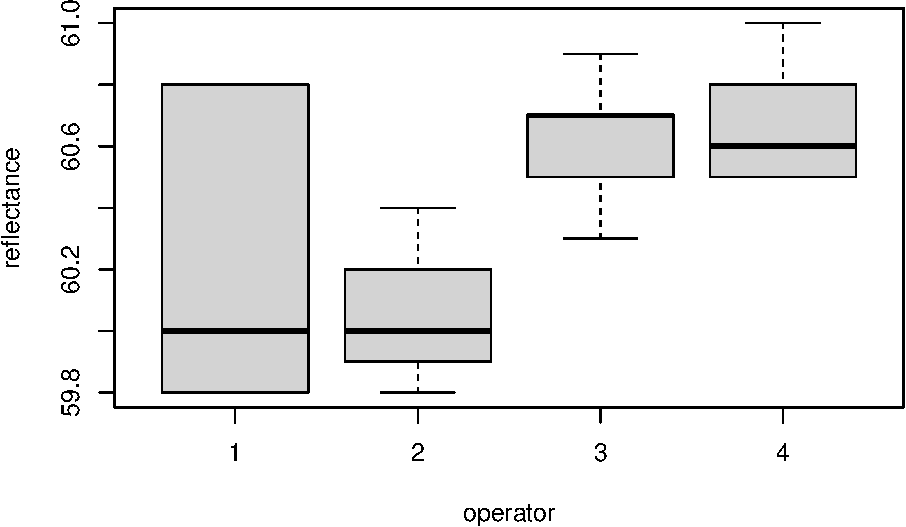
\includegraphics{bookdown_math3014-6027_files/figure-latex/pulp-boxplot-1} 

}

\caption{Pulp experiments: distributions of reflectance from the four operators.}\label{fig:pulp-boxplot}
\end{figure}

Figure \ref{fig:pulp-boxplot} shows that, relative to the variation, there may be a difference in the mean response between treatments 1 and 2, and 3 and 4. In this chapter, we will see how to make this comparison formally using linear models, and to assess how the choice of design impacts our results.

\end{example}

Throughout this chapter we will assume the \(i\)th treatment is applied to \(n_i\) experimental unit, with total number of runs \(n = \sum_{i=1}^t n_i\) in the experiment.

\hypertarget{a-unit-treatment-linear-model}{%
\section{A unit-treatment linear model}\label{a-unit-treatment-linear-model}}

An appropriate, and common, model to describe data from such experiments when the response is continuous is given by

\begin{equation}
y_{ij} = \mu + \tau_i + \varepsilon_{ij}\,, \quad i = 1, \ldots, t; j = 1, \ldots, n_i\,, 
\label{eq:utm}
\end{equation}

where \(y_{ij}\) is the response from the \(j\)th application of treatment \(i\), \(\mu\) is a constant parameter, \(\tau_i\) is the effect of the \(i\)th treatment, and \(\varepsilon_{ij}\) is the random individual effect from each experimental unit with \(E(\varepsilon_{ij})\) and \(\mathrm{Var}(\varepsilon_{ij}) = \sigma^2\). All random errors are assumed independent and here we also assume \(\varepsilon_{ij} \sim N(0, \sigma^2)\).

Model \eqref{eq:utm} assumes that each treatment can be randomly allocated to one of the \(n\) experimental units, and that this allocation is independent of the allocation of all the other treatments.

Why is this model appropriate and commonly used? The expected response from the application of the \(i\)th treatment is

\[
E(y_{ij}) = \mu + \tau_i\,.
\]
The parameter \(\mu\) can be thought of as representing the impact of many different features particular to \textbf{this} experiment, and \(\tau_i\) is the deviation due to applying treatment \(i\). From the applicable of two different hypothetical experiments, A and B, the expected response from treatment \(i\) may be different due to a different overall mean. From experiment A:

\[
E(y_{ij}) = \mu_{\mathrm{A}} + \tau_i\,.
\]
From experiment B:
\[
E(y_{ij}) = \mu_{\mathrm{B}} + \tau_i\,.
\]
But the \textbf{difference} between treatments \(k\) and \(l\) (\(k, l = 1,\ldots, t\))

\begin{align*}
E(y_{kj}) - E(y_{lj}) & = \mu_A + \tau_k - \mu_A - \tau_l \\
& = \tau_k - \tau_l\,,
\end{align*}

is constant across different experiments. This concept of \textbf{comparison} underpins most design of experiments, and will be applied throughout this module.

\hypertarget{the-partitioned-linear-model}{%
\section{The partitioned linear model}\label{the-partitioned-linear-model}}

In matrix form, we can write model \eqref{eq:utm} as

\[
\boldsymbol{y}= X_1\mu + X_2\boldsymbol{\tau}+ \boldsymbol{\varepsilon}\,,
\]
where \(X_1 = \boldsymbol{1}_n\), the \(n\)-vector with every entry equal to one,

\[
X_2 = \begin{bmatrix}
\boldsymbol{1}_{n_1} & \boldsymbol{0}_{n_1} & \cdots &  \boldsymbol{0}_{n_1} \\
\boldsymbol{0}_{n_2} & \boldsymbol{1}_{n_2} & \cdots &  \boldsymbol{0}_{n_2} \\
\vdots & & \ddots & \vdots \\
\boldsymbol{0}_{n_t} & \boldsymbol{0}_{n_t} & \cdots &  \boldsymbol{1}_{n_t} \\
\end{bmatrix}\,,
\]
with \(\boldsymbol{0}_{n_i}\) is the \(n_i\)-vector with every entry equal to zero, \(\boldsymbol{\tau}= [\tau_1, \ldots, \tau_t]^{\mathrm{T}}\) and \(\boldsymbol{\varepsilon}= [\varepsilon_{11}, \ldots, \varepsilon_{tn_t}]^{\mathrm{T}}\).

Why are we partitioning the model? Going back to our discussion of the role of \(\mu\) and \(\tau_i\), it is clear that we not interested in estimating \(\mu\), which represents an experiment-specific contribution to the expected mean. Our only interest is in estimating the (differences between the) \(\tau_i\). Hence, we can treat \(\mu\) as a nuisance parameter.

If we define \(X = [X_1\, \vert\, X_2]\) and \(\boldsymbol{\beta}^{\mathrm{T}} = [\mu \vert \boldsymbol{\tau}^{\mathrm{T}}]\), we can write the usual least squares equations

\begin{equation}
X^{\mathrm{T}}X\hat{\boldsymbol{\beta}} = X^{\mathrm{T}}\boldsymbol{y}
\label{eq:crd-ls}
\end{equation}
as a system of two matrix equations

\begin{align*}
X_1^{\mathrm{T}}X_1\hat{\mu} + X_1^{\mathrm{T}}X_2\hat{\boldsymbol{\tau}} & = X_1^{\mathrm{T}}\boldsymbol{y}\\
X_2^{\mathrm{T}}X_1\hat{\mu} + X_2^{\mathrm{T}}X_2\hat{\boldsymbol{\tau}} & = X_2^{\mathrm{T}}\boldsymbol{y}\,. \\
\end{align*}

Assuming \((X_1^{\mathrm{T}}X_1)^{-1}\) exists, which it does in this case, we can pre-multiply the first of these equations by \(X_2^{\mathrm{T}}X_1(X_1^{\mathrm{T}}X_1)^{-1}\) and subtract it from the second equation to obtain

\begin{align*}
X_2^{\mathrm{T}}[I_n - X_1(X_1^{\mathrm{T}}X_1)^{-1}X_1^{\mathrm{T}}]X_1\hat{\mu} 
& + X_2^{\mathrm{T}}[I_n - X_1(X_1^{\mathrm{T}}X_1)^{-1}X_1^{\mathrm{T}}]X_2\hat{\boldsymbol{\tau}} \\
& = X_2^{\mathrm{T}}[I_n - X_1(X_1^{\mathrm{T}}X_1)^{-1}X_1^{\mathrm{T}}]\boldsymbol{y}\,.
\end{align*}

Writing \(H_1 = X_1(X_1^{\mathrm{T}}X_1)^{-1}X_1^{\mathrm{T}}\), we obtain

\begin{equation}
X_2^{\mathrm{T}}[I_n - H_1]X_1\hat{\mu} + X_2^{\mathrm{T}}[I_n - H_1]X_2\hat{\boldsymbol{\tau}} = X_2^{\mathrm{T}}[I_n - H_1]\boldsymbol{y}\,.
\label{eq:almost-reduced}
\end{equation}
The matrix \(H_1\) is a ``hat'' matrix for a linear model containing only the term \(\mu\), and hence \(H_1X_1 = X_1\) (see MATH2010). Hence the first term in \eqref{eq:almost-reduced} is zero, and we obtain the \textbf{reduced normal equations} for \(\boldsymbol{\tau}\):

\begin{equation}
X_2^{\mathrm{T}}[I_n - H_1]X_2\hat{\boldsymbol{\tau}} = X_2^{\mathrm{T}}[I_n - H_1]\boldsymbol{y}\,.
\label{eq:crd-red-normal}
\end{equation}

Note that the solutions from \eqref{eq:crd-red-normal} are not different from the solution to \(\hat{\boldsymbol{\tau}}\) that would be obtained from solving \eqref{eq:crd-ls}; equation \eqref{eq:crd-red-normal} is simply a re-expression, where we have eliminated the nuisance parameter \(\mu\). This fact means that we rarely need to solve \eqref{eq:crd-red-normal} explicitly.

Recalling that for a hat matrix, \(I_n - H_1\) is idempotent and symmetric (see MATH2010), if we define

\[
X_{2|1} = (I_n - H_1)X_2\,,
\]
then we can rewrite equation \eqref{eq:crd-red-normal} as

\begin{equation}
X_{2|1}^{\mathrm{T}}X_{2|1}\hat{\boldsymbol{\tau}} = X_{2|1}^{\mathrm{T}}\boldsymbol{y}\,, 
\label{eq:rne}
\end{equation}

which are the normal equations for a linear model with expectation \(E(\boldsymbol{y}) = X_{2|1}\boldsymbol{\tau}\).

For the CRD discussed in this chapter, \(X_1^{\mathrm{T}}X_1 = n\), the total number of runs in the experiment\footnote{In later chapters we will see examples where \(X_1\) has \(>1\) columns, and hence \(X_1^{\mathrm{T}}X_1\) is a matrix.}. Hence \((X_1^{\mathrm{T}}X_1)^{-1} = 1/n\) and \(H_1 = \frac{1}{n}J_n\), with \(J_n\) the \(n\times n\) matrix with all entries equal to 1.

The adjusted model matrix then has the form

\begin{align*}
X_{2|1} & = (I_n - H_1)X_2 \\
& = X_2 - \frac{1}{n}J_nX_2 \\
& = X_2 - \frac{1}{n}[n_1\boldsymbol{1}_n \vert \cdots \vert n_t\boldsymbol{1}_n]\,. 
\end{align*}

That is, every column of \(X_2\) has been adjusted by the subtraction of the column mean from each entry\footnote{Often called ``column centred''}. Also notice that each row of \(X_{2|1}\) has a row-sum equal to zero (\(= 1 - \sum_{i=1}^tn_t/n\)). Hence, \(X_{2|1}\) is not of full column rank, and so the reduced normal equations do not have a unique solution\footnote{If we recalled the material on ``dummy'' variables from MATH2010 chapter 5, we would already have realised this.}.

In MATH2010 we fitted models with categorical variables by defining a set of dummy variables and estimating a reduced model. Here, we will take a slightly different approach and study which combinations of parameters from \eqref{eq:utm} are estimable, and in particular which linear combinations of the treatment parameters \(\tau_i\) we can estimate. We start with a short digression to discuss the concept of a generalised inverse.

\hypertarget{generalised-inverses}{%
\section{Generalised inverses}\label{generalised-inverses}}

A generalised inverse of a square, symmetric matrix \(A\) is any matrix \(A^{-}\) that satisfies

\[
AA^{-}A = A\,.
\]

If matrix \(A\) is of full column rank, then there is a single generalised inverse \(A^{-} = A^{-1}\), the usual inverse matrix. In other cases, there may be infinitely many choices for \(A^{-}\).

\hypertarget{solutions-to-the-reduced-normal-equations}{%
\section{Solutions to the reduced normal equations}\label{solutions-to-the-reduced-normal-equations}}

We can use a generalised inverse to generate solutions to \eqref{eq:rne} of the form:

\[
\hat{\boldsymbol{\tau}} = (X_{2|1}^{\mathrm{T}}X_{2|1})^{-}X_{2|1}^{\mathrm{T}}\boldsymbol{y}\,.
\]
Substituting this expression into \eqref{eq:rne}, we obtain

\begin{align*}
X_{2|1}^{\mathrm{T}}X_{2|1}(X_{2|1}^{\mathrm{T}}X_{2|1})^{-}X_{2|1}^{\mathrm{T}}\boldsymbol{y}& = X_{2|1}^{\mathrm{T}}H_{2|1}\boldsymbol{y}\\ 
& = X_{2|1}^{\mathrm{T}}\boldsymbol{y}\,,
\end{align*}

where \(H_{2|1} = X_{2|1}(X_{2|1}^{\mathrm{T}}X_{2|1})^{-}X_{2|1}^{\mathrm{T}}\) and \(X_{2|1}^{\mathrm{T}}H_{2|1} = X^{\mathrm{T}}_{21}\)\footnote{This equality follows from \(H\) being the projection matrix for the column space of \(X\).}.

\hypertarget{blocking}{%
\chapter{Blocking}\label{blocking}}

\hypertarget{factorial}{%
\chapter{Factorial experiments}\label{factorial}}

\hypertarget{blocking-in-factorial-designs}{%
\chapter{Blocking in factorial designs}\label{blocking-in-factorial-designs}}

\hypertarget{fractional-factorial-designs}{%
\chapter{Fractional factorial designs}\label{fractional-factorial-designs}}

\hypertarget{response-surface-methodology}{%
\chapter{Response surface methodology}\label{response-surface-methodology}}

\hypertarget{optimal-design-of-experiments}{%
\chapter{Optimal design of experiments}\label{optimal-design-of-experiments}}

  \bibliography{math3014-6027.bib,packages.bib}

\end{document}
